\documentclass{beamer}
\usetheme{CMU}

\usepackage{pgf,pgfarrows,pgfnodes,pgfautomata,pgfheaps,pgfshade}
\usepackage{amsmath,amssymb}
\usepackage[utf8]{inputenc}
\usepackage{colortbl}
\usepackage[english]{babel}
\usepackage{booktabs}
\usepackage{slpython}
\usepackage{underscore}

\author{Luís Pedro Coelho}
\institute{Programming for Scientists}

\graphicspath{{figures/}{figures/generated/}{images/}}

\newcommand*{\code}[1]{\textsl{#1}}


\title{Databases for Large Amounts of Data}
\begin{document}
\frame{\maketitle}

\begin{frame}[fragile]
\frametitle{Databases}

For large amounts of data (thousands or millions of records).

\end{frame}

\begin{frame}[fragile]
\frametitle{Example Databases}

\begin{block}{Traditional}

\begin{itemize}
\item MySQL (open source)
\item Postgres (open source)
\item Oracle
\item MS-SQL
\item \ldots
\end{itemize}
\end{block}

\begin{block}{Non-traditional}
\begin{itemize}
\item SQLite (open source)
\item Pytable [HDF5] (open source)
\item MS-Access
\item \ldots
\end{itemize}
\end{block}
\end{frame}

\begin{frame}[fragile]
\frametitle{Traditional Databases}

\begin{block}{Two Processes}
\begin{enumerate}
\item Application
\item Database
\end{enumerate}
\end{block}

\note{They not even need to be on the same machine.}
\end{frame}

\begin{frame}[fragile]
\frametitle{Relational Databases}

\begin{itemize}
\item Based on relations
\item Relational database management system (RDMS)
\end{itemize}

\end{frame}

\begin{frame}[fragile]

\centering
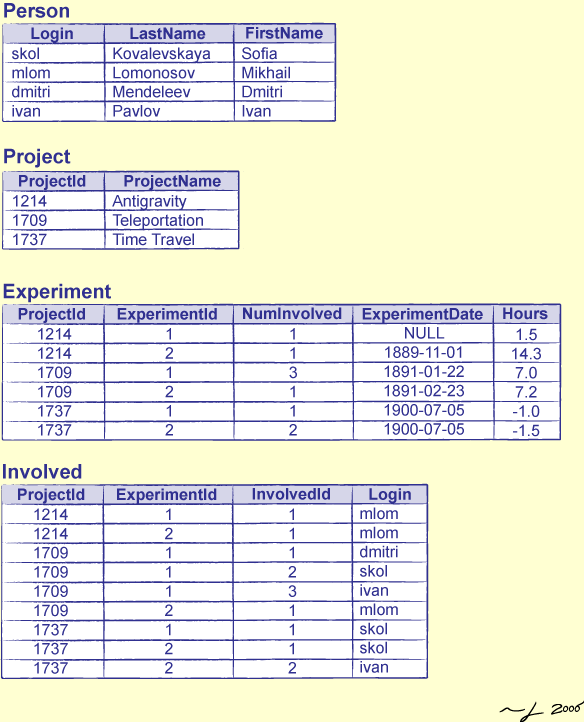
\includegraphics[height=.9\textheight]{11-db-example}

\creditto{Software Carpentry Website}
\note{Use this image to discuss 
    (1) keys
    (2) foreign keys
}

\end{frame}

\begin{frame}[fragile]
\frametitle{Join}
\begin{columns}
\column[t]{.5\textwidth}
Users

\centering
\begin{tabular}{lll}
\textbf{Username} & \textbf{Name} & \textbf{Email} \\
\midrule
lpc & Lu\'\i s & lpc@cmu\\
rita & Rita & rita@yahoo\\
\ldots\\
\end{tabular}
\column[t]{.5\textwidth}
Content

\centering
\begin{tabular}{lll}
\textbf{Page} & \textbf{Username} & \textbf{Date} \\
\midrule
index & lpc & 2008-12-12\\
slides & rita &  2009-2-8\\
project & lpc & 2009-3-20\\
\ldots\\
\end{tabular}
\end{columns}

\pause
\bigskip
\bigskip
\bigskip
\begin{tabular}{lll}
\textbf{Page} & \textbf{Username} & \textbf{Email} \\
\midrule
index & lpc & lpc@cmu.edu\\
slides & rita &  rita@yahoo.com\\
project & lpc & lpc@cmu.edu\\
\ldots\\
\end{tabular}
\end{frame}

\begin{frame}[fragile]

DRY: Don't Repeat Yourself\\
a.k.a.\ Single Point of Truth

\note{This is actually a good software engineering principle, but I haven't had an opportunity to mention 'til today.}
\end{frame}

\begin{frame}[fragile]
\frametitle{SQL: The language of Databases}

\alert{SQL}: Structured Query Language.\\
The standard way to access databases.\\

\medskip
(At least for some meanings of the word \alert{standard}).
\note{97\% of SQL is standard. The other 3\% are enough to cause problems.}
\end{frame}

\begin{frame}[fragile]
\frametitle{SQL: Example}
\begin{verbatim}
CREATE TABLE users (
    username VARCHAR(255) PRIMARY KEY,
    user VARCHAR(255) NOT NULL,
    email VARCHAR(255)
    );
\end{verbatim}
\end{frame}

\begin{frame}[fragile]
\frametitle{Create table}

\texttt{CREATE} \textit{tablename} (\\
    \textit{name} \textit{type} \textit{modifiers},\\
    \ldots);
\end{frame}

\begin{frame}[fragile]
\frametitle{Selects}

\begin{verbatim}
SELECT pages.page, users.username, users.email
FROM pages, users
WHERE pages.username = users.username;
\end{verbatim}

\end{frame}
\begin{frame}[fragile]

\begin{columns}
\column[t]{.5\textwidth}
Users

\centering
\begin{tabular}{lll}
\textbf{Username} & \textbf{Name} & \textbf{Email} \\
\midrule
lpc & Lu\'\i s & lpc@cmu\\
rita & Rita & rita@yahoo\\
\ldots\\
\end{tabular}
\column[t]{.5\textwidth}
Content

\centering
\begin{tabular}{lll}
\textbf{Page} & \textbf{Username} & \textbf{Date} \\
\midrule
index & lpc & 2008-12-12\\
slides & rita &  2009-2-8\\
project & lpc & 2009-3-20\\
\ldots\\
\end{tabular}
\end{columns}

\pause
\texttt{SELECT *}\\
\texttt{FROM users, pages}\\
\uncover<4->{\texttt{WHERE users.username = pages.username};}
\pause

\begin{tabular}{llllll}
\textbf{users.U} & \textbf{users.N} & \textbf{users.E} & \textbf{page.P} & \textbf{page.U} & \textbf{pages.D} \\
\midrule
lpc & Lu\'\i s & lpc@cmu & index & lpc & 2008-12-12\\
\only<3>{lpc & Lu\'\i s & lpc@cmu & slides & rita &  2009-2-8\\}
lpc & Lu\'\i s & lpc@cmu & project & lpc & 2009-3-20\\
\only<3>{rita & Rita & rita@yahoo & index & lpc & 2008-12-12\\}
rita & Rita & rita@yahoo & slides & rita &  2009-2-8\\
\only<3>{rita & Rita & rita@yahoo & project & lpc & 2009-3-20\\}
\ldots
\end{tabular}
\end{frame}

\begin{frame}[fragile]
\frametitle{In Practice}

SQL is a \alert{declarative} language:\\
you declare what you want \alert{not how to do it}.

\end{frame}

\begin{frame}[fragile]
\frametitle{Select Statement}

\texttt{SELECT} \textit{*} or \textit{column names}\\
\texttt{FROM} \textit{dabasases}\\
\texttt{WHERE} \textit{conditions}

\end{frame}

\begin{frame}[fragile]
\frametitle{Conditions}

\begin{verbatim}
SELECT COUNT(*)
FROM users, pages
WHERE users.username = pages.username AND
    date > DATE('2008-12-31')
    ;
\end{verbatim}
\end{frame}

\begin{frame}[fragile]
\frametitle{What's a NULL?}

A NULL is a special object that represents \alert{missing}.

\note{Often you will want your tables to not have NULLs.

NULL is a bit like a NaN.
}
\end{frame}

\begin{frame}[fragile]
\frametitle{Foreign Key}
We had a \textit{Page.Username} which is foreign key into Users.

\begin{verbatim}
CREATE TABLE Pages (
    Name VARCHAR(255) NOT NULL,
    Username VARCHAR(255) NOT NULL FOREIGN KEY(Users),
    ...);
\end{verbatim}
\end{frame}

\begin{frame}[fragile]
\frametitle{Other Commands: INSERT}

\begin{verbatim}
INSERT INTO pages
    VALUES('new-page','lpc',DATE('2009-3-31'));
\end{verbatim}

\end{frame}

\begin{frame}[fragile]
\frametitle{Other Commands: UPDATE}

\begin{verbatim}
UPDATE pages
    SET username = 'rita'
    WHERE name = 'index'
\end{verbatim}

\end{frame}

\begin{frame}[fragile]
\frametitle{Other Commands: DELETE}

\texttt{DELETE FROM} \textit{table}\\
\texttt{WHERE} \textit{condition};

\end{frame}

\begin{frame}[fragile]
\frametitle{What We'll Talk About on Thursday}

\begin{itemize}
\item How to set up a simple database (sqlite)
\item Non-traditional databases (pytables)
\end{itemize}
\end{frame}

\end{document}
